
\chapter[Approach]{Approach}
\graphicspath{ {images/approach} }

In this chapter we will present an approach that produce a visual and auditive depiction of the evolution of a system. 
Our approach consists of two parts: 
In the first part we modelled the evolution of the software artifacts, and we enginereed a tool that implement it.
In the second part, we used the concept of synesthesia (the production of a sense impression relating to one sense by stimulation of another sense) 
to enhance the effectiveness of the visualization. 

\section{Evolutionary model}
Analyzing the evolution of a systems requires to consider numerous aspects. 
In our approach we focus on systems that resides on git repositories. 
We made this choiche because git is the most common repository management system and it also track all the changes made to the system.
As a consequence we can use it to reconstruct the history of a system.\\

In our approach, we model the evolution of repository files, therefore we model its history. 
To do that, we considered all the information that can be extracted from a git repository: files and commits.

The git protocol is responsible for tracking the changes made to the system.
To do that, every time we made a commit, it stores only a list of files that have been modified. 
Every commit is represented by a tree of hashes, each one representing a file. 

Git has the possibility to inspect every commit of a repository by using the command \texttt{git checkout}. 
In this way, we can navigate through the history of a repository, to track all the files, their changes and their metrics.\\

A commit operation contains also other meta-information such as the author, the date and the message. 

We built our model on the top of the Lanza's \i{evolution matrix} \cite{Lanza2001} with some adoption to work well with the git protocol. 
We represented the history of a repository as a matrix with the following properties:
\begin{itemize}
    \item Each column of the matrix represent a commit, a version of the software.
    \item Each row of the matrix represent a file, named FileHistory.
    \item Each cell of the matrix represent the different versions of a file. Empty cells represent a file that has not been modified.
    \item A file can have multiple names (tollerant to renaming and moving operations).
    \item Files are sorted by addition time, on the top we will have all the files that were added in the first commit of the repository. 
\end{itemize}

For now on, we will use the following notation:
\begin{itemize}
    \item A \textbf{FileHistory} represents a row of the matrix.
    \item A \textbf{ProjectVersion} represents a column of the matrix.
    \item A \textbf{FileVersion} represents a cell of the matrix.
\end{itemize}

Therefore, a FileHisory represents the history of an entity of our system. 
The name of the file is not a concern for us, until a file is not deleted it will always represent the same entity. 

Git it smart enought to recognize five types of changes:
\begin{itemize}
    \item \textbf{Add}: a file is added in the repository.
    \item \textbf{Delete}: a file is deleted in the repository.
    \item \textbf{Modify}: a file is modified in the repository.
    \item \textbf{Rename}: a file is renamed in the repository.
    \item \textbf{Move}: a file is moved in the repository.
\end{itemize}

And we will use them in our model to identify the action associated to a FileVersion. 
\begin{figure}
    \center
    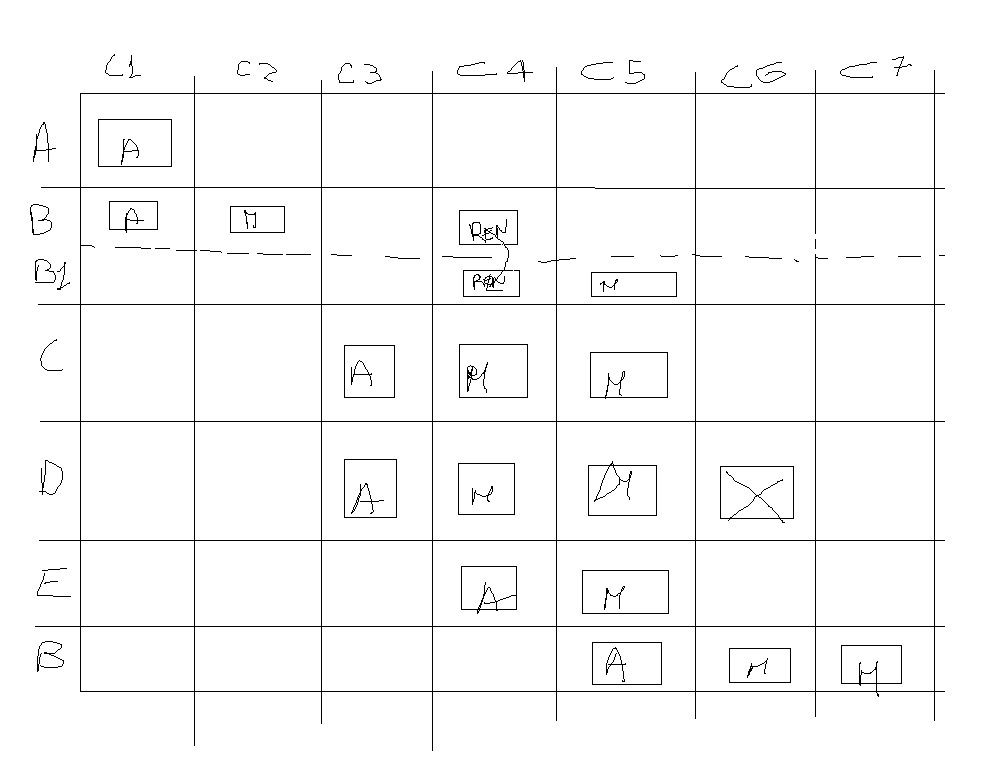
\includegraphics[width=0.6\textwidth]{ApproachMatrix.jpg}
    \caption{Evolution matrix of a repository}
    \label{fig:evolutionMatrixApproach}
\end{figure}
Figure \ref{fig:evolutionMatrixApproach} present a schematic evolution matrix of a repository with seven versions.
As we can see, in the first ProjectVersion, there were added two files, A and B. In the second revision B was modified, and in the third revision C and D were added.
The fourth revision recorded a rename of B to B1.
It's important to notice that B and B1 represent the same entity, therefore they are represented by the same FileHistory.\\



Based on our aim, we can read this matrix as follows:
 \begin{itemize}
     \item \textbf{by rows}, if we are intrested on the history of a particular entity of our system. 
     For examle, the FileHistory represented by the first third row in figure \ref{fig:evolutionMatrixApproach}, represents the history of the file D. 
     The file D was added in the third ProjectVersion (so the third commit), modified in the fourth and fifth ProjectVersion, and then deleted in the sixth ProjectVersion.
     The figure \ref{fig:evolutionMatrixApproach} is also a good exaple to understand why we cannot rely on the name of the file to identify the entity. 
     We can notice that the file B represented by the second FileHistory, was added on the first version and then renamed on the fourth from B to B1. 
     Then, in the fifth version, a new file called B was added. Nonetheless the name of the files are the same, they must represent two different entity. 
     We would have had the same result, even if the file B was been added in the version four. 
     \item \textbf{by columns}, if we are intrested on which entities were updated on each ProjectVersion. 
    For example, on the first ProjectVersion we have added the first and the second entity. 
    On the fourth ProjectVersion we have renamed the second entity, we have modified both the third and the fourth, and finally we have added the fifth entity.
 \end{itemize}

\begin{figure}
    \center
    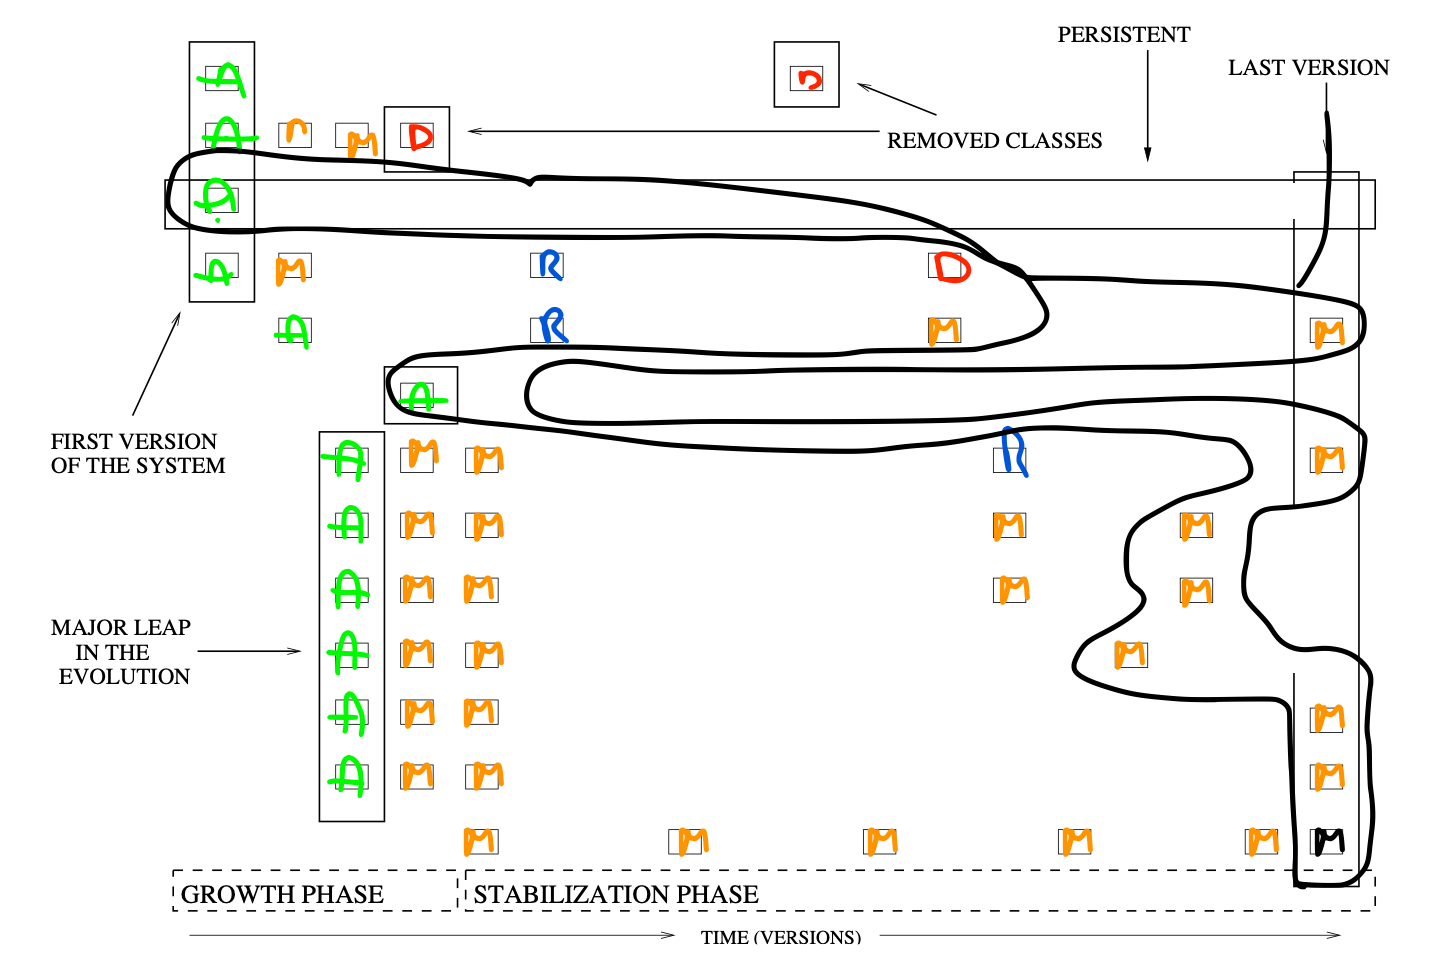
\includegraphics[width=\textwidth]{ApproachMatrix2.png}
    \caption{Evolution matrix of a repository}
    \label{fig:evolutionMatrixApproach2}
\end{figure}

Figure  \ref{fig:evolutionMatrixApproach2} shows an exaple of how to recover evolution information from the matrix. 
As we have seen, each version doesn not represent a snapshot of the system.
Instead it represents only the differentce in term of changes made to the previous version. 
Given that, to recover a snapshot of a specific version, we need to consider the last changes made before that specific version.
Under those circumstances, for each FileHistory, we need to go back in time until we find the leftmost change. Of course, if the leftmost change was a delete, we have to ignore the releated FileHistory.
In contrast, if we have to display the evolution of a snapshot, we need to consider only the changes made after that snapshot. 
So, each time we need to display a ProjectVersion, we have to take all its FileVersions and merge them with the current state of the snapshot. 

\section{Visualization model}

Software systems are hard to understand due to the complexity and the sheer size of the data to be analyzed.
Our approach aims to make the analysis of a system easier and more for the engineers, through the exploitation of the human senses.
This is the reason why we have chosen to leverage on the phenomenom of the Synesthesia.
The phenomenon of the synesthesia occurs  when a stimulation of a sense or a cognitive pathway leads to the involountarly stimuation of another sense or a cognitive pathway.
We experience synesthesia when two or more things are perceived as the same. 
For exaple, synesthetic people might associate the red color with the letter D or the green color with the letter A. 
There are many forms of synesthesia, each one representing a different type of perception, such as visual forms, auditory, tactile, etc.\\
\\
In our approach we use the following visual aspects to trigger involountarly associations:
\begin{itemize}
    \item \textbf{Color}: we use the color of the entity to describe the last action made on that entity.
    \item \textbf{Shape}: we use the shape of the entity to describe the type of the entity. 
    For exaple, a java file could be represented by a cube whereas a binary file could be represented by a sphere.
    \item \textbf{Height}: we use the height of the entity to describe the value of a representative metric, used to compare entities.
\end{itemize}

Entities are displayed with an outward spiral layout to emphatize their order on the evolution matrix. \\

There are several ways to traverse the history of a repository. 
The visualization needs to start from the first moment and then go forward until the end. The question is, how we should go forward in time?
We came up with two strategies: 
\begin{itemize}
    \item We can display \texttt{n} version at time, so we are traversing the history as it was written. 
    A limitation of this approach is that we lose the concept of time. 
    We cannot have any idea about how much time was passed between two commit, thus we cannot distinguish active development phases from unactive development phases. 

    \item We can group version by their timestamp. So, all the commit made in the sime time period, will be displayed at the same time. 
    This strategy works very well if we need to comphrend how the system evolved and at which speed in time. 
\end{itemize}

We conchretized our strategies witht the concept of \textbf{moment}. A moment is a group of version that will be displayed at the same time. 


\begin{figure}[H]
    \begin{center}
        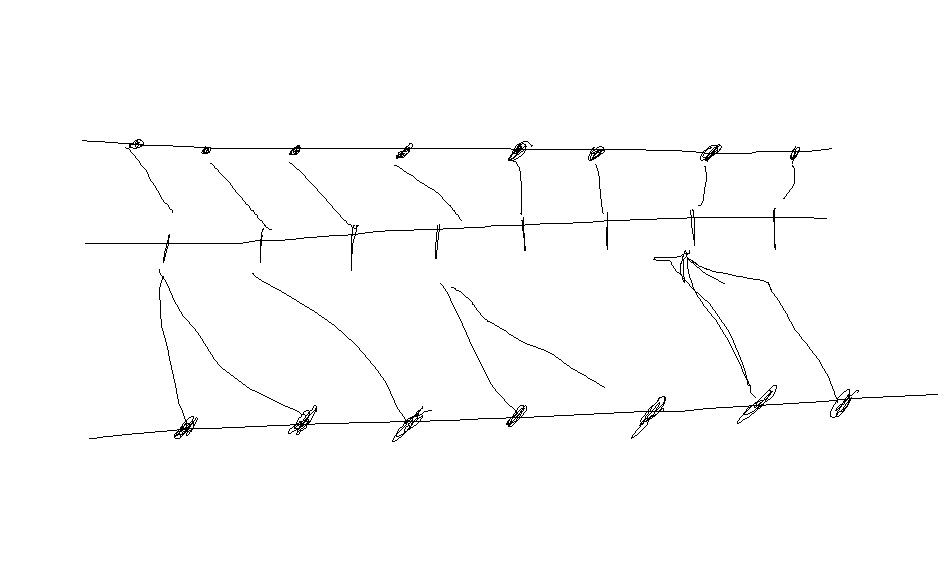
\includegraphics[width=0.9\linewidth]{Moments.jpg} 
        \caption{Example of two different strategies to identity moments. 
        On the first strategy, we mapped one commit with one moment, so the total number of moments will be equals to the total number of commit.  
        Alternatively, on the second strategy, we created a moment every day.
        As a result, we have some moments with many commits, and some without anyone.
        With this strategy, the number of moments will be the same as the number of days that have passed between the first and the last commit. 
        }
        \label{fig:moment}
    \end{center}
\end{figure}

Figure \ref{fig:moment} highlights the difference between the two strategies mentioned above. 


\subsection*{Color}


\begin{wrapfigure}{r}{0.3\textwidth}
    \begin{center}
        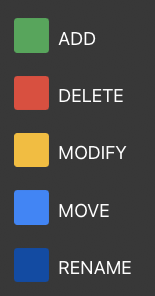
\includegraphics[width=0.7\linewidth]{ColorAssociation.png} 
        \caption{Color association}
        \label{fig:ColorAssociation}
    \end{center}
\end{wrapfigure}

The color of the entity should recall the last action made on that entity. To achieve this purpose, we used the color association described in figure \ref{fig:ColorAssociation}
Nonetheless each person has its own perception, we can not assume that this color will work in the same way for all the pepoles.
To remedy this issue, users can customize the color palette as they wish. \\

Moreover, we decided to put another information on the color of the entity: the \textbf{aging}. 
We define the aging of an entity as the number of moments since the last modification of that entity happened.
To do that, we mapped the age of an entity with the darkness of its color. 
As a result, older entities will be displayed with a darker color. 
In this way, users can immediately recognize the last action and the amount of time passed since the entity was modified.


\subsection*{Shape}
The shape of the entity defines the type of the entity itself. 
It should be something fully customizable by the user, so it can chose on which entity he can focus on. 

\subsection*{Height}
The height of an entity should represent the value of a metric.


\section{Auditive model}